\documentclass[11pt]{article}
\usepackage{iitbtitle}
\usepackage{caption}
\usepackage{subcaption}
\usepackage{a4wide}
\usepackage{multirow}
\usepackage{anysize}
\usepackage{iitbcs}
\usepackage{latexsym}
\usepackage{amssymb}
\usepackage{amsmath}
\usepackage{graphicx}
\usepackage{epsfig}
\usepackage{comment}
% \usepackage{psfig}
\usepackage{tabls}
\usepackage{multirow}
\usepackage{tabularx}
\usepackage{url}
\newcolumntype{Y}{>{\centering\arraybackslash}X}
\setlength{\floatsep}{7pt plus 2pt minus 2pt}
\setlength{\textfloatsep}{5pt plus 2pt minus 2pt}
\setlength{\intextsep}{5pt plus 2pt minus 2pt}
\usepackage{color}

\marginsize{2.5cm}{2.5cm}{1cm}{1.5cm}
\def\baselinestretch{1.15}

\newcommand\INPUT{\item[\textbf{Input:}]}
\newcommand\OUTPUT{\item[\textbf{Output:}]}
\providecommand{\norm}[1]{\lVert#1\rVert}
\DeclareGraphicsExtensions{.pdf,.png,.jpg}
\begin{document}


%\baselineskip 20pt
%The definitions
\def\title{Quadcopter Based Applications in Imaging}
\def\what{Third Annual Progress Report}
\def\degree{Doctor of Philosophy}
\def\who{Meghshyam G. Prasad}
\def\roll{124058001}
\def\guide{Prof. Sharat Chandran \\ Prof. Michael Brown}
\titlpage
\def\bsq{\begin{flushright} $\blacksquare$\\ \end{flushright}}
\def\tab{\hspace{5mm}}

\newpage
\section*{Acknowledgements}
I express deep and sincere gratitude to Prof. Sharat Chandran and Prof.
Michael Brown for providing constant direction and guidance. I am also
very much grateful to Prof. David Hsu for giving me access to his lab and
equipments. I am also thankful to Mr. Abhishek Chakrborty and Mr. Ravi Chalasani
for their help in stangnant water detection project.

\begin{flushright}
Meghshyam G. Prasad
\end{flushright}

\pagenumbering{roman}
\newpage
\begin{abstract}
In today's world, digital imaging is being extensively used in almost all
sectors. In some situations, it is quite difficult to take pictures from
handheld camera. Low cost quadcopters such as Parrot's AR Drone may be used in
such scenarios to take photos of an object which is otherwise out of reach of normal
camera. There are two problems involved in it: first to track the given object
and second to take ``good'' pictures of it. In my last APS we discussed 
about the first problem. Here, we will see how to take good pictures and use it for
variouos applications.

One of the use case where we may use quadcopter for imaging is to
capture a panaroma of big wall (or any such planar object). In such cases, it
will be very tedious and tiring to use hand held camera. Secondly, if there are
vacant spaces on a wall, it is challenging for existing mosaicing techniques as
there will be little to no features to match input images. So, in our work, we
focuses on a method to construct panoramas captured from a quadcopter, that
consists of scenes with significant regions of vacant spaces.

We describe a framework that is able to handle this unique input by
leveraging the availability of the inertial measurement unit (IMU)
data from the quadcopter that is synchronized with the input images.
We use the IMU data for two purposes: first to select images which can
be stiched together. Second, in combination with coarse stereo reconstruction,
we determine appropriate portions of the images to complete the panorama. We
demonstrate the efficacy of our approach on a number of input sequences that
cannot to be mosaiced by existing methods.

After using quadcopter for mosaicing of images, we thought of using it for 
some ``survey'' application. In recent times, there has been a sharp increase
in dengue and malaria, especially in urban areas. One of the major reasons for
this health hazard is the number of locations where one can find stagnant
water. These locations are large breeding ground for fast multiplying
mosquitoes, and other insects. Areas include traditionally uncovered gutters,
and also terraces of high rise buildings, and shades above windows (popularly
known as chhajja)-- areas that are hard to reach and access. We propose the use
of a quadcopter to inspect areas and identify stagnant water patches.  Water
being specular in nature tends to confound traditional image processing
methods. Further the use of a non-traditional camera mounted on a quadcopter
presents new challenges.  We provide methods to get past such hurdles.

\noindent \textbf{Keywords:} Quadcopter, Panoramic Image Stitching, Stagnant Water Detection

\end{abstract}
\newpage
\pagenumbering{arabic}
\tableofcontents

%\begingroup\def\thispagestyle#1{}\def\baselinestretch{1.5}\tableofcontents\endgroup
\newpage

\section{Motivation}
\section{Introduction}
\section{Mosaicing Scenes with Vacant Spaces}
\begin{figure}[h!]
  \centering
  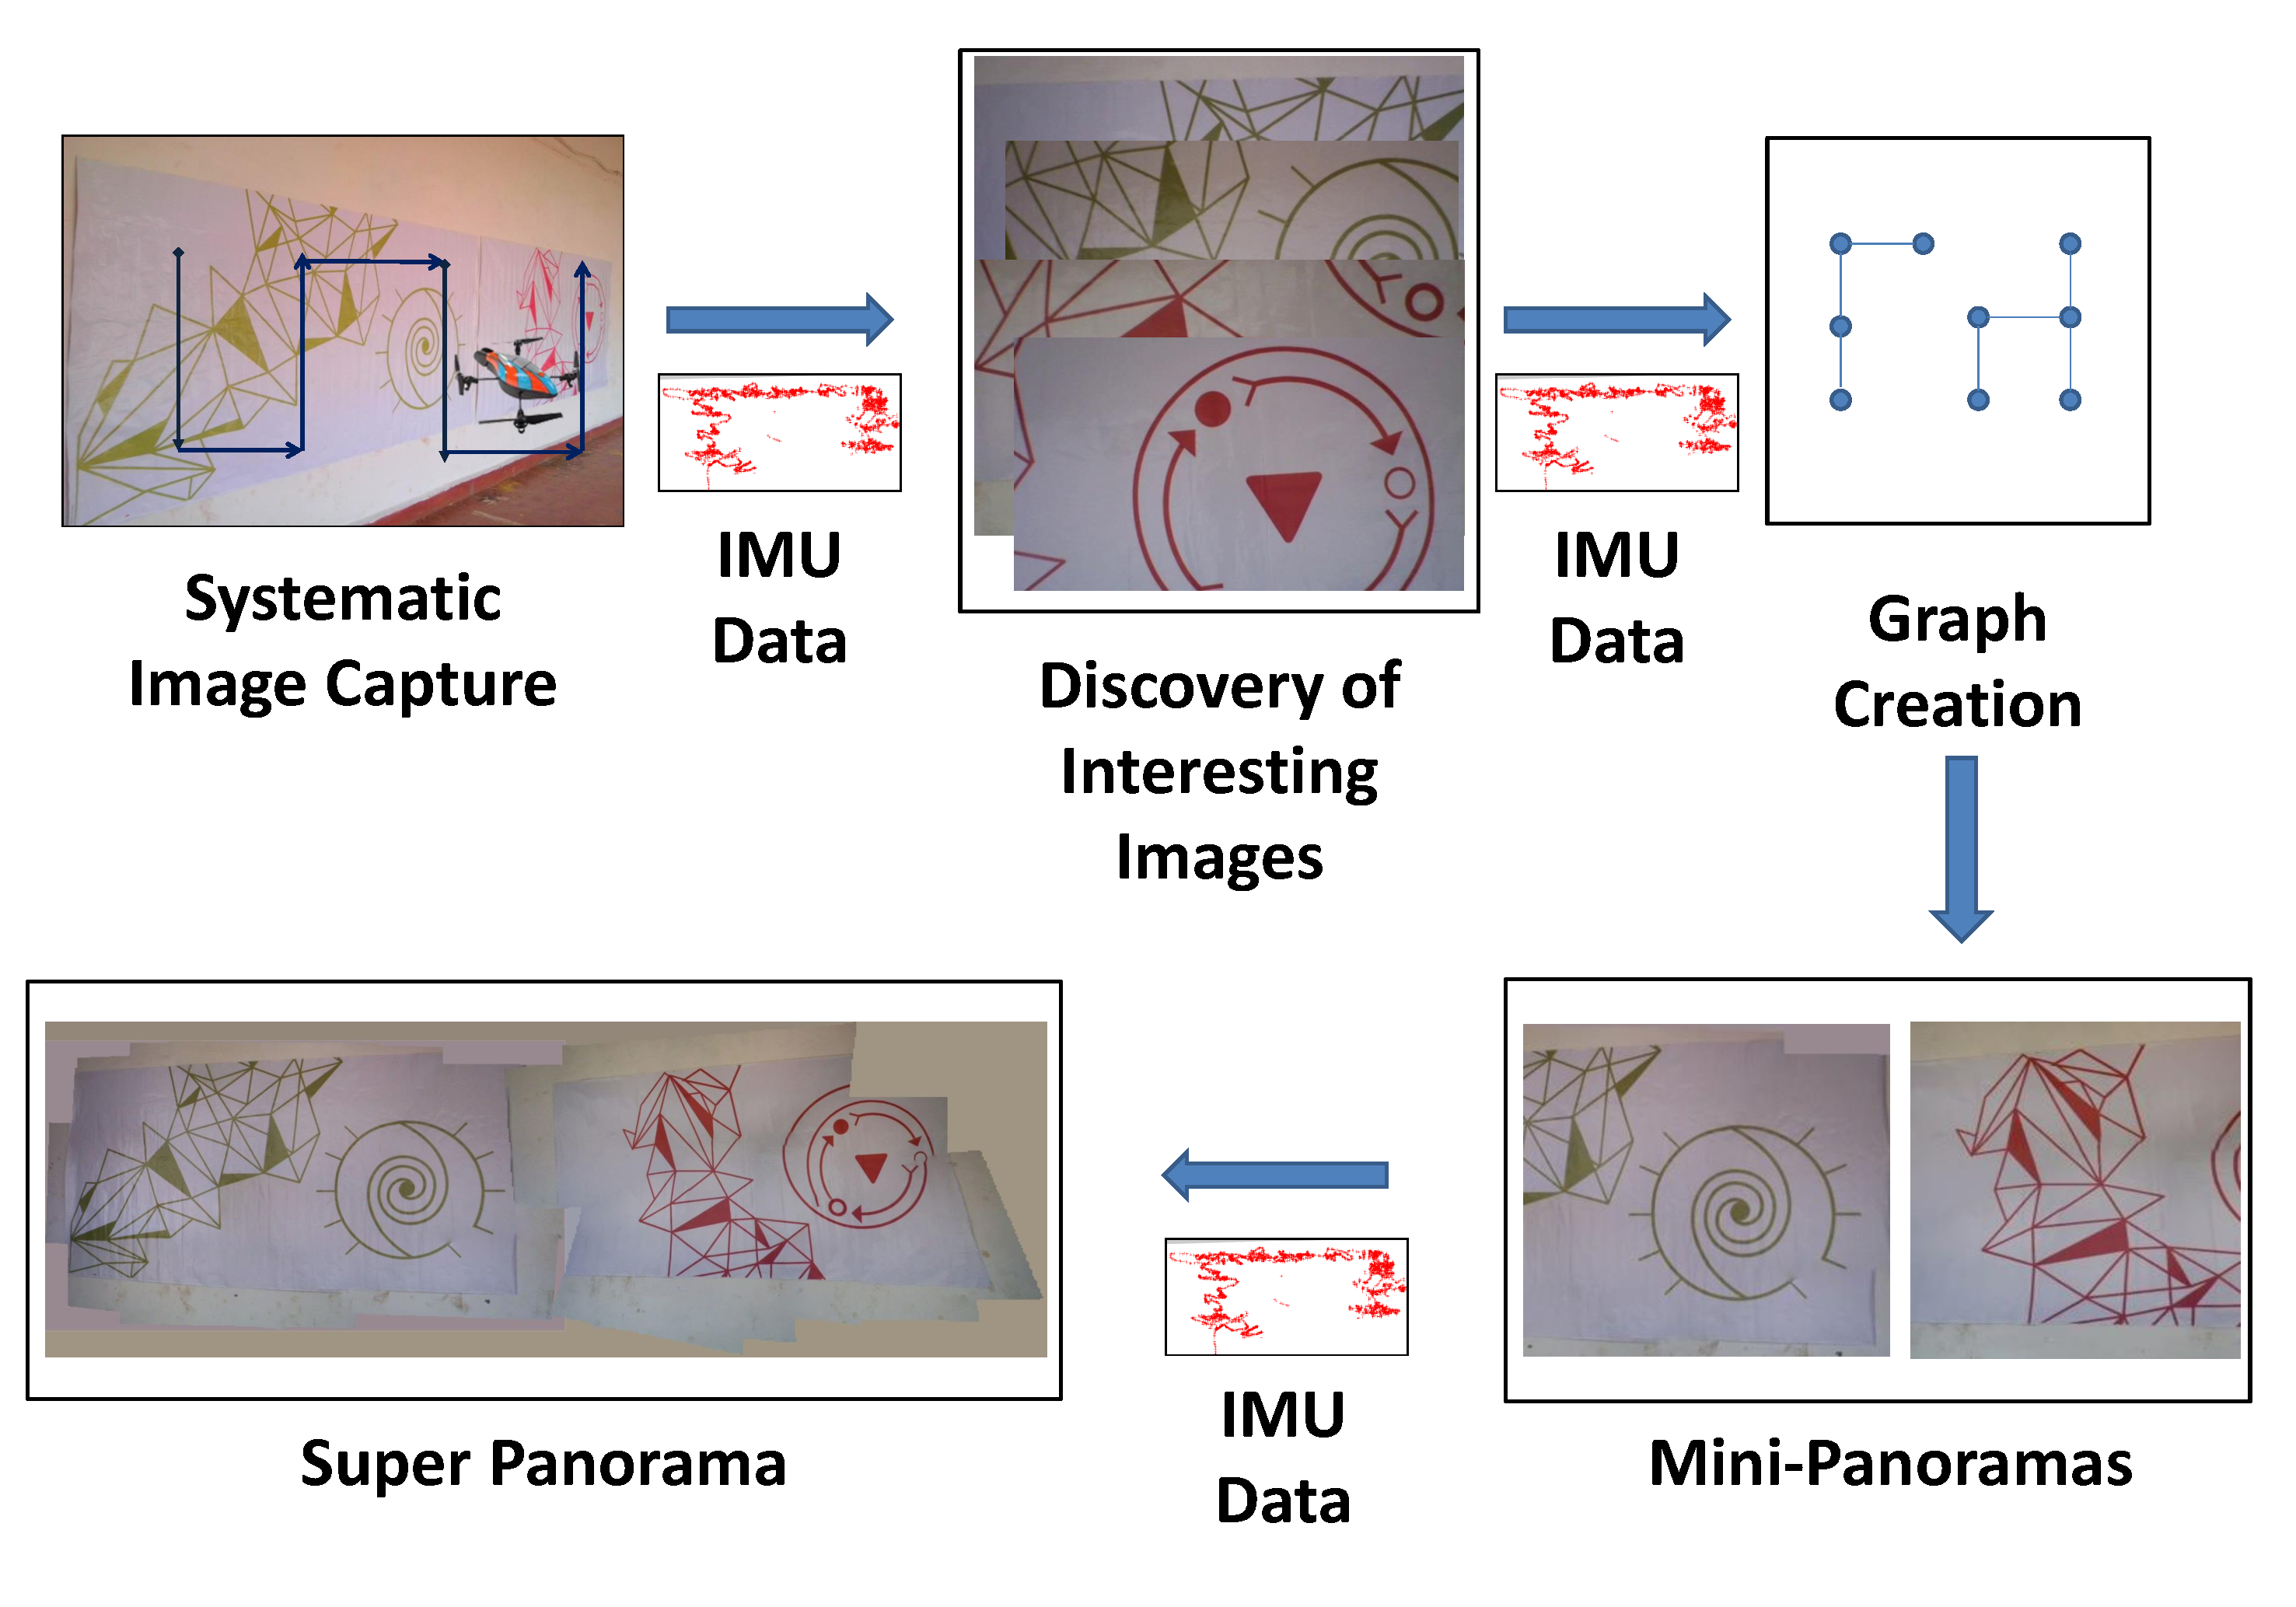
\includegraphics[width=\textwidth]{figures/Workflow} 
  \caption{ \label{fig:workflow} Overview: Input imagery is
    systematically acquired (top left) by a quadcopter.  In the next
    step, interesting images are found by clustering the video into
    regions based on positional data.  A graph is constructed using
    proximal images. For each connected component in a graph, standard
    stitching techniques are used to create mini-panoramas which are
    then joined together into super panorama 
    again using IMU data.}
\end{figure}
\subsection{Path Planning}
\subsection{Multi-planar Cases}

\section{Quadcopter-based Stagnant Water Identification}

\begin{figure}[h!]
  \centering
  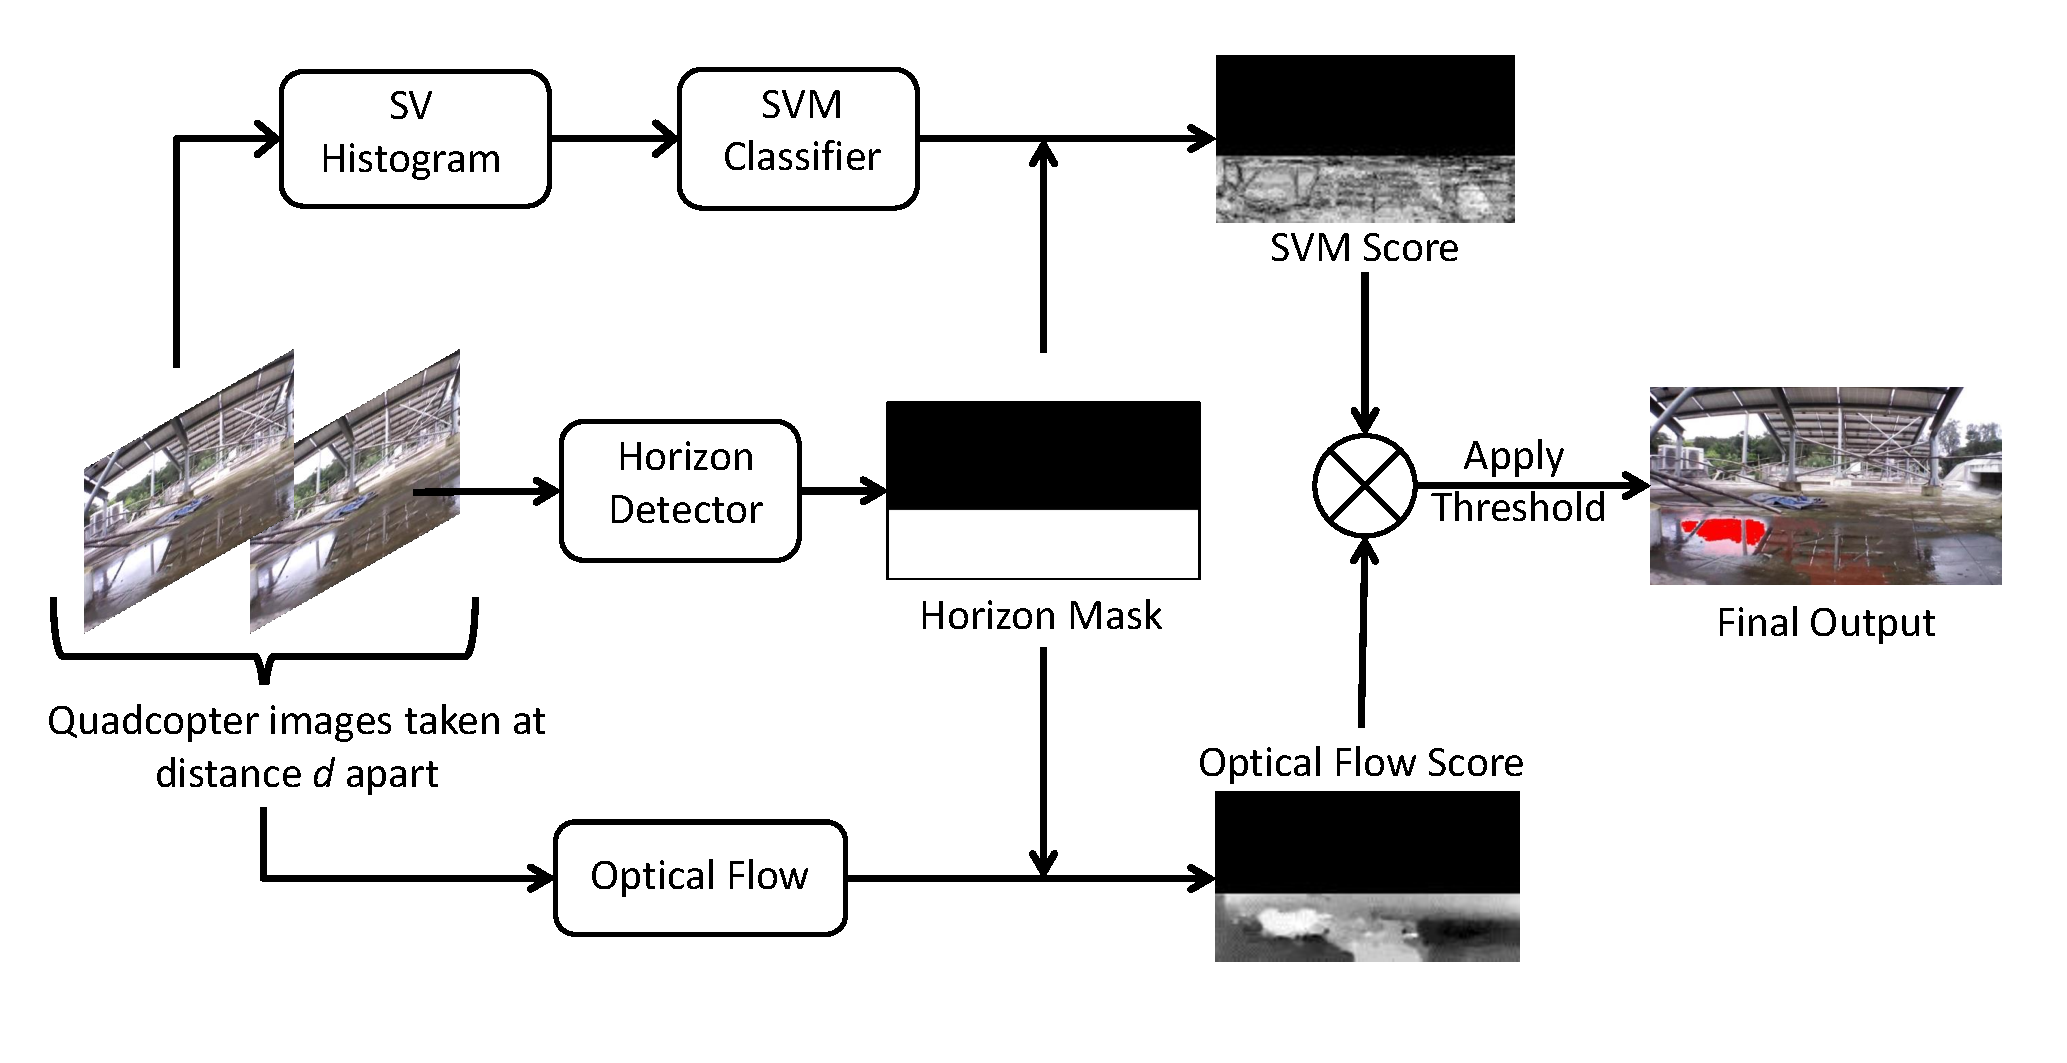
\includegraphics[width=\textwidth]{figures/overall_workflow.pdf}
  \caption{Overall architecture.}
  \label{fig:workflow}
\end{figure}

\newpage

\end{document}
